\documentclass[10pt,a4paper,titlepage,oneside]{article}
\usepackage{LabProtocol}

\exercise{Exercise II}

% enter your data here
\authors{
	Mihai-Andrei Dancu, Matr. Nr. 12123694 \par
	{\small e12123694@student.tuwien.ac.at} \par
}


\begin{document}

\maketitle


%████████╗ █████╗ ███████╗██╗  ██╗     ██╗
%╚══██╔══╝██╔══██╗██╔════╝██║ ██╔╝    ███║
%   ██║   ███████║███████╗█████╔╝     ╚██║
%   ██║   ██╔══██║╚════██║██╔═██╗      ██║
%   ██║   ██║  ██║███████║██║  ██╗     ██║
%   ╚═╝   ╚═╝  ╚═╝╚══════╝╚═╝  ╚═╝     ╚═╝
\Task{Space Invaders Game}

\begin{qa}{Briefly describe the architecture of your \textsf{game} module. Are there any submodules? What is their purpose? How many FSMs did you use? (approximately 6-8 sentences, you can also include figures)}

	My game module architecture is implemented using a single FSM with multiple states, which can broadly be categorised in a number of pseudo-states. These are the \textbf{reset and init} state 
	(where the bitmaps are created and the double frame buffering is implemented), the \textbf{movement of the game objects and collision detection} (player, invaders, shots), the \textbf{drawing of text} 
	(the pause menu, game over menu or the score and number of lives left) and the \textbf{drawing of the actual game objects} (player, invaders, shots, bunkers). I have used the following submodule: 
	\textbf{shot\_ctrl} for the drawing of shots, \textbf{sifield} for managing the space invaders field and \textbf{decimal\_printer} which converts the current score to ASCII printable, readable
	digits. \textbf{Figure 1} shows the operations per frame of the game that the FSM executes. Moreover, I created the \textbf{mygame\_pkg} package to keep the source file cleaner and shorter.

	\begin{figure}[h!]
		\centering
		\includegraphics[width=0.75\linewidth]{dia/pdf/game_op_per_frame.pdf}
		\caption{Operations per frame}
	\end{figure}
\end{qa}


%%%%%%%%%%%%%%%%%%%%%%%%%%%%%%%%%%%%%%%%%%%%%%%%%%%%%%%%%%%%%%%%%%%%%%%%%%%%%%%%


%████████╗ █████╗ ███████╗██╗  ██╗    ██████╗ 
%╚══██╔══╝██╔══██╗██╔════╝██║ ██╔╝    ╚════██╗
%   ██║   ███████║███████╗█████╔╝      █████╔╝
%   ██║   ██╔══██║╚════██║██╔═██╗     ██╔═══╝ 
%   ██║   ██║  ██║███████║██║  ██╗    ███████╗
%   ╚═╝   ╚═╝  ╚═╝╚══════╝╚═╝  ╚═╝    ╚══════╝
\Task{DualShock Controller}


\begin{qa}{Oscilloscope Measurements}

	As can be seen in \textbf{Figure 2} on the right side the square and circle buttons were pressed and the left stick x axis displacement is 80 while the y axis displacement is ff.
	\textbf{Figure 3} shows a more clear view of the measured signals which are to be decoded to see if the results match the state from Figure 2. The results can be seen in the table below
	and they indeed match the controller state.

	\begin{figure}[h!]
		\centering
		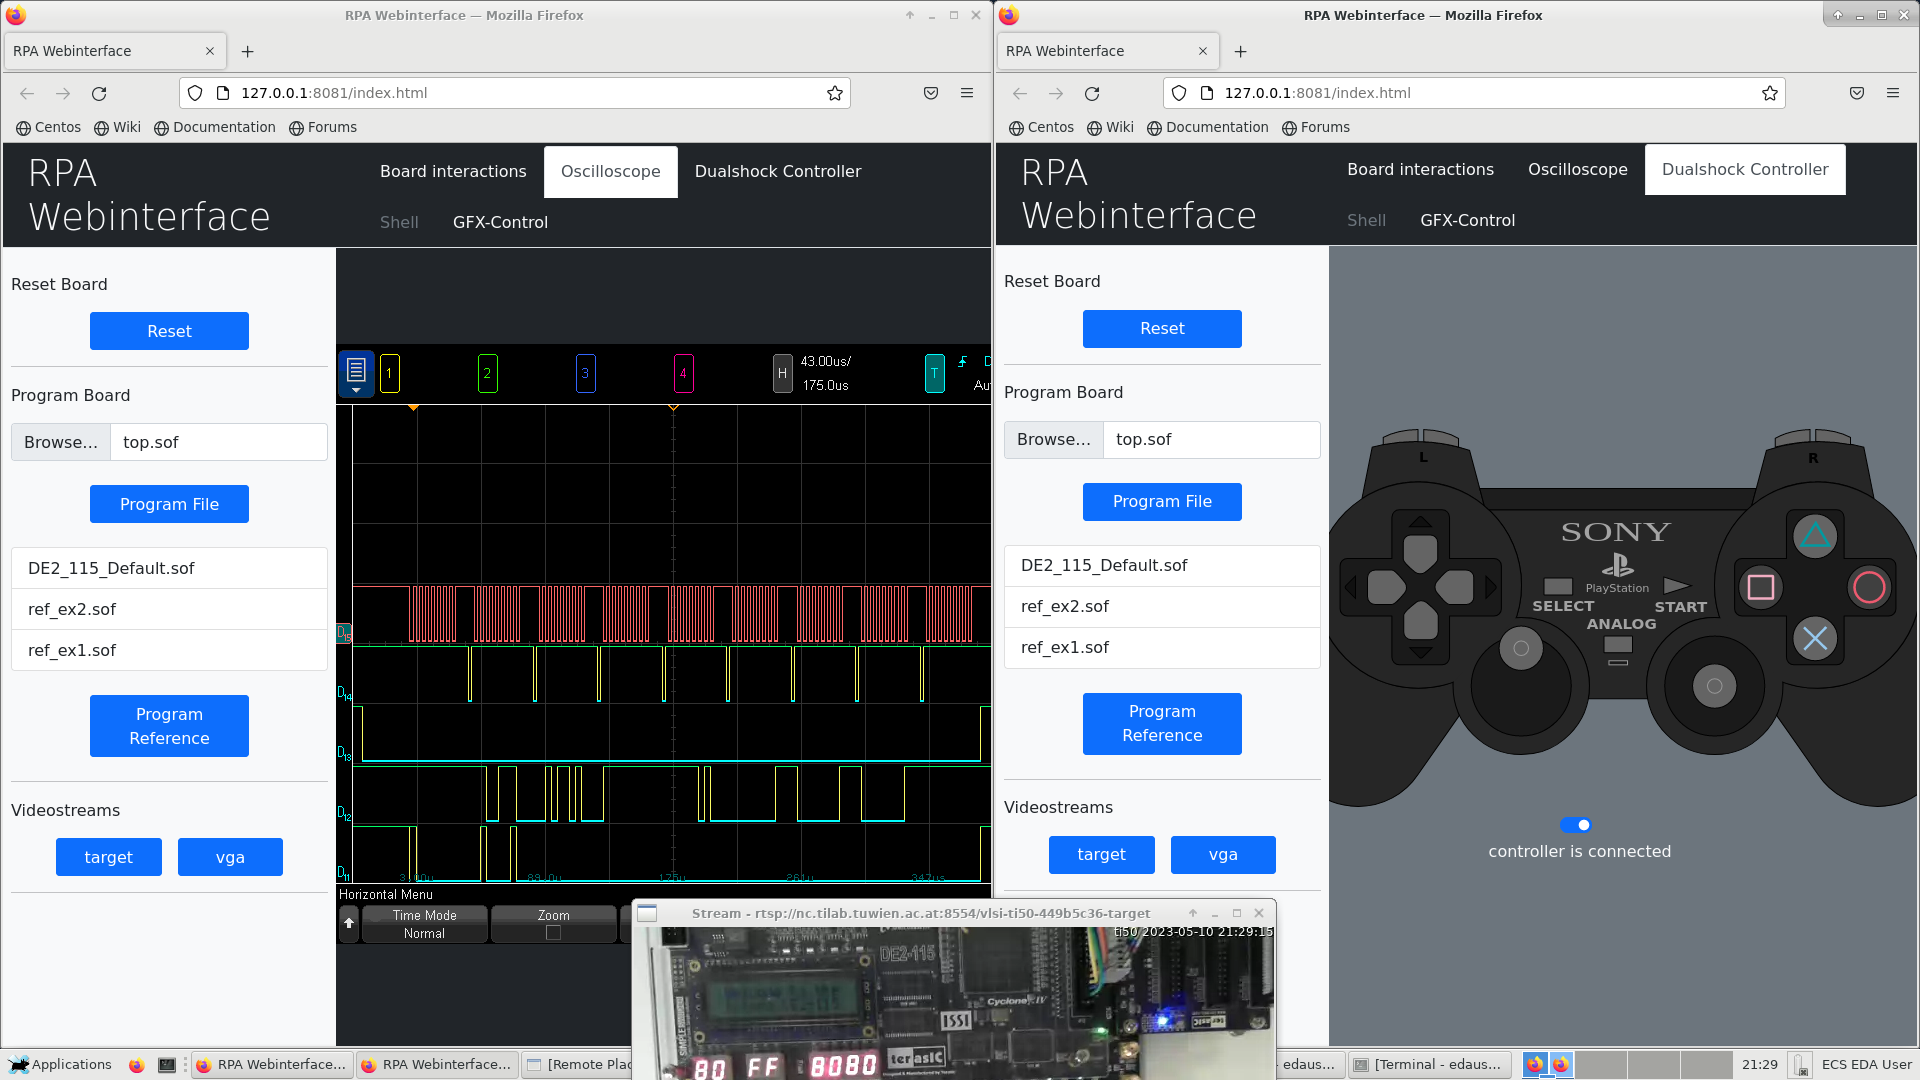
\includegraphics[width=0.75\linewidth]{complete.png}
		\caption{Controller state}
	\end{figure}

	\begin{figure}[h!]
		\centering
		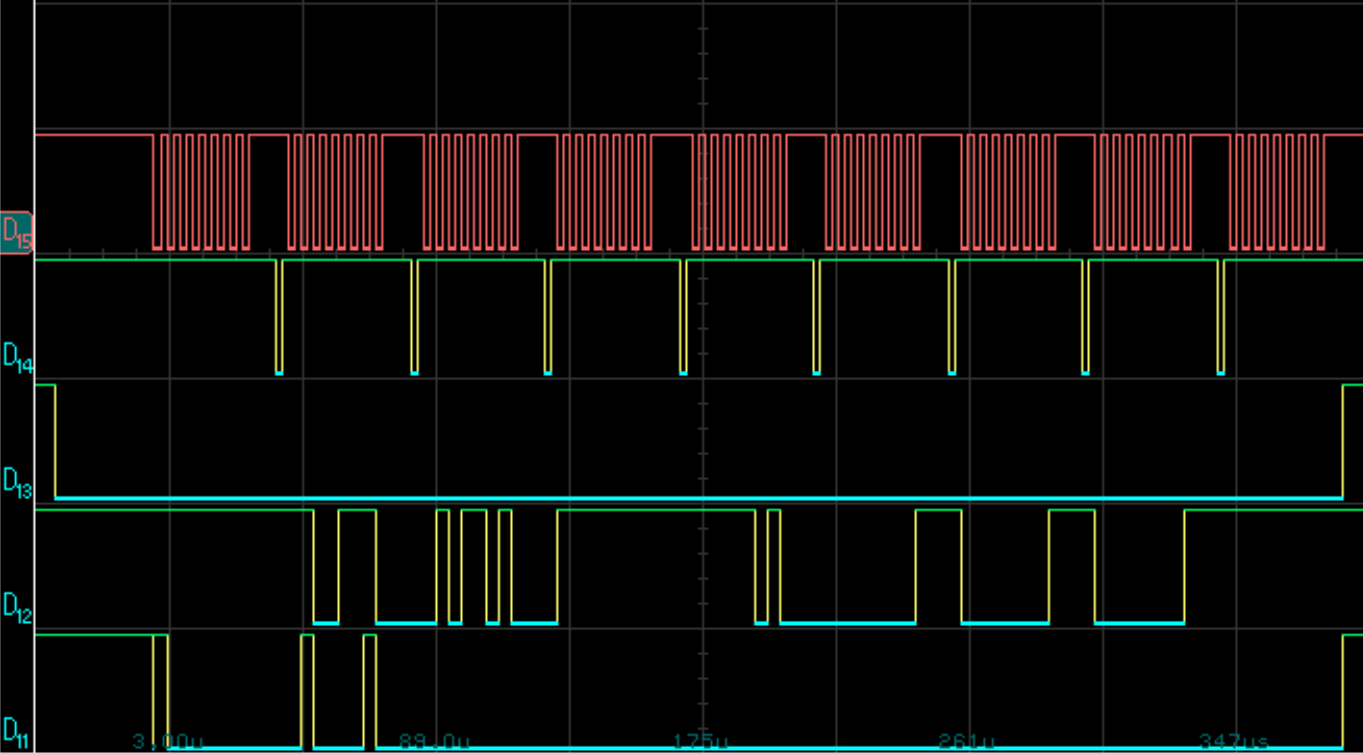
\includegraphics[width=0.75\linewidth]{zoomed.png}
		\caption{Measured signals}
	\end{figure}

	\begin{center}

	\begin{center}
	\ttfamily
	\begin{tabular}{|l|l|l|l|l|l|l|l|l|l|}
	\hline
	byte    & 1    & 2    & 3    & 4     & 5     & 6     & 7     & 8     & 9    \\ \hline
	command & 0x01 & 0x42 & 0x00 & 0x00  & 0x00  & 0x00  & 0x00  & 0x00  & 0x00 \\ \hline
	data    & 0xff & 0x73 & 0x5a & 0xff  & 0x5f  & 0x01  & 0x01  & 0x01  & 0xff \\ \hline
	\end{tabular}
	\end{center}
	\end{center}

\end{qa}


%%%%%%%%%%%%%%%%%%%%%%%%%%%%%%%%%%%%%%%%%%%%%%%%%%%%%%%%%%%%%%%%%%%%%%%%%%%%%%%%

%████████╗ █████╗ ███████╗██╗  ██╗    ██████╗ 
%╚══██╔══╝██╔══██╗██╔════╝██║ ██╔╝    ╚════██╗
%   ██║   ███████║███████╗█████╔╝      █████╔╝
%   ██║   ██╔══██║╚════██║██╔═██╗      ╚═══██╗
%   ██║   ██║  ██║███████║██║  ██╗    ██████╔╝
%   ╚═╝   ╚═╝  ╚═╝╚══════╝╚═╝  ╚═╝    ╚═════╝ 
\Task{Bonus: SignalTap Measurement}

\begin{qa}{Trigger Condition}
	\begin{figure}[h!]
		\centering
		% \includegraphics[width=1.0\linewidth]{your filename here}
		\dummyimage
		\caption{Screenshot showing the trigger condition}
	\end{figure}
\end{qa}
%%%%%%%%%%%%%%%%%%%%%%%%%%%%%%%%%%%%%%%%%%%%%%%%%%%%%%%%%%%%%%%%%%%%%%%%%%%%%%%%

\begin{qa}{Measurement Screenshot}
	\begin{figure}[h!]
		\centering
		% \includegraphics[width=1.0\linewidth]{your filename here}
		\dummyimage
		\caption{Screenshot showing ths signal traces of one of the response time measurements}
	\end{figure}
\end{qa}
%%%%%%%%%%%%%%%%%%%%%%%%%%%%%%%%%%%%%%%%%%%%%%%%%%%%%%%%%%%%%%%%%%%%%%%%%%%%%%%%

\begin{qa}{Response Time Measurement}
\begin{center}
\begin{tabular}{|l|c|c|c|c|c|c|c|c|c|}
	\hline
	Measurement   & 1 & 2 & 3 & 4 & 5 & 6 & 7 & 8\\\hline
	Response time &   &   &   &   &   &   &   &  \\\hline
\end{tabular}
\end{center}
\end{qa}
%%%%%%%%%%%%%%%%%%%%%%%%%%%%%%%%%%%%%%%%%%%%%%%%%%%%%%%%%%%%%%%%%%%%%%%%%%%%%%%%


\begin{qa}{Why is the response time not a constant value? What do you think contributes to it?}

\end{qa}
%%%%%%%%%%%%%%%%%%%%%%%%%%%%%%%%%%%%%%%%%%%%%%%%%%%%%%%%%%%%%%%%%%%%%%%%%%%%%%%%

\end{document}
